%%%%%%%%%%%%%%%%%%%%%%%%%%%%%%%%%%%%%%%%%%%%%%%%%%%%%%%%%%%%%%%%%%%%%%%%%%%

\documentclass[a4paper,oneside,12pt]{article}
\usepackage{mystyle}

\begin{document}

\title{\Large\bf Conic sections}
\author{%%
  Minh Van Nguyen \\
  \url{mvngu@gmx.com}
}
\date{\today}
\maketitle


%%%%%%%%%%%%%%%%%%%%%%%%%%%%%%%%%%%%%%%%%%%%%%%%%%%%%%%%%%%%%%%%%%%%%%%%%%%

\section{How to program a robot}

At 06:58 UTC on 04th December 1996, the National Aeronautics and Space
Administration~(NASA) of the USA launched a spacecraft called the Mars
Pathfinder.\footnote{
  See the following website for further information:
  \url{http://web.archive.org/web/20180729201819/https://www.jpl.nasa.gov/missions/details.php?id=5913}.
}
The destination of the spacecraft was the planet Mars.  On 04th July
1997, the spacecraft landed on Mars.  The mission had one primary
objective: to study the Red Planet.  This task was performed by a
robotic rover called Sojourner, which explored the surface of Mars for
$85$ Earth days.\footnote{
  You can read about the results sent back to Earth by Sojourner in
  the paper at
  \url{http://web.archive.org/web/20180729072504/http://science.sciencemag.org/content/sci/278/5344/1758.full.pdf}.
}

\begin{figure}[!htbp]
\centering
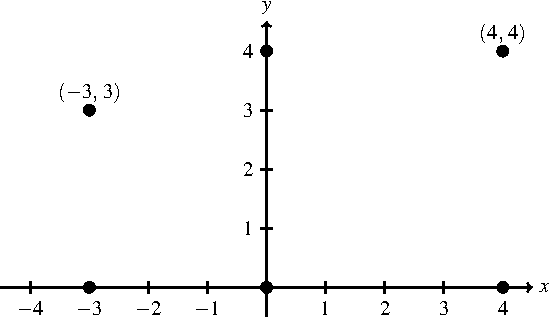
\includegraphics[scale=1.1]{image/14/robot-path-points.pdf}
\caption{%%
  Points on a flat surface.  A robot is initially placed at the
  origin.  How would you program the robot to visit all the given
  points?
}
\label{fig:conic:robot_points}
\end{figure}

How would you program a robot such as Sojourner to move around a flat
surface?  One way is to interpret each location of the flat surface as
a point $\tuple{x}{y}$ in the Cartesian coordinate system.  The
$x$-coordinate would tell the robot to move in the east-west
direction.  The $y$-coordinate would tell the robot to move in the
north-south direction.  As an example, consider the points in
\Figure{fig:conic:robot_points} and suppose that the robot is
initially placed at the point $\tuple{0}{0}$.  How would you program
the robot to visit all of the given points and finally arrive at its
original location?  You can specify the points in the order in which
the robot is to visit the points.  Suppose that you specify the path
of the robot as the points in the sequence
%%
\begin{equation}
\label{eqn:conic:robot_path_sequence}
\tuple{0}{0}\comma
\tuple{4}{0}\comma
\tuple{4}{4}\comma
\tuple{0}{4}\comma
\tuple{0}{0}\comma
\tuple{-3}{-3}\comma
\tuple{-3}{0}\comma
\tuple{0}{0}.
\end{equation}
%%
The sequence~\eqref{eqn:conic:robot_path_sequence} means that the
robot starts off at the point $\tuple{0}{0}$ and travels directly to
the point $\tuple{4}{0}$.  From $\tuple{4}{0}$ the robot then travels
directly to $\tuple{4}{4}$.  And so on until the robot arrives at its
original location of $\tuple{0}{0}$.
\Figure{fig:conic:robot_path_square_triangle} illustrates the path of
the robot as given by the points in the
sequence~\eqref{eqn:conic:robot_path_sequence}.

\begin{figure}[!htbp]
\centering
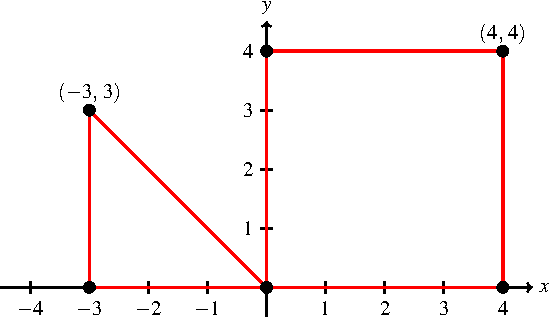
\includegraphics[scale=1.1]{image/14/robot-path-square-triangle.pdf}
\caption{%%
  A robot is initially placed at the origin.  The red lines highlight
  the path of the robot, where the path is given by the points in the
  sequence~\eqref{eqn:conic:robot_path_sequence}.
}
\label{fig:conic:robot_path_square_triangle}
\end{figure}

\begin{exercise}
\textbf{Another path.}
Consider the points in \Figure{fig:conic:robot_points}.  A robot is
initially placed at the origin.  The path of the robot is given by the
sequence of points:
%%
\begin{equation}
\label{eqn:conic:robot_another_path_sequence}
\tuple{0}{0}\comma
\tuple{0}{4}\comma
\tuple{-3}{3}\comma
\tuple{-3}{0}\comma
\tuple{0}{0}\comma
\tuple{4}{4}\comma
\tuple{4}{0}\comma
\tuple{0}{0}.
\end{equation}
%%
Use the points in the
sequence~\eqref{eqn:conic:robot_another_path_sequence} to trace out
the path of the robot.
\end{exercise}

\ifbool{showSolution}{
\begin{solution}
See \Figure{fig:conic:robot_another_path}.

\begin{figure}[!htbp]
\centering
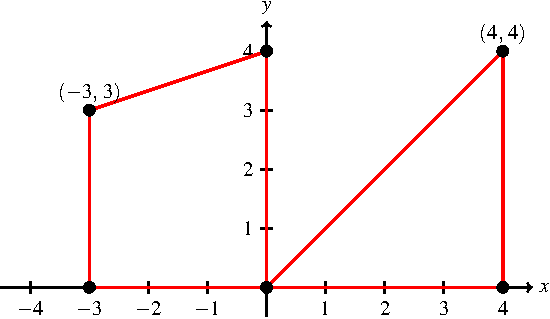
\includegraphics[scale=1.1]{image/14/robot-path-quad-triangle.pdf}
\caption{%%
  A robot is initially placed at the origin.  The red lines highlight
  the path of the robot, where the path is given by the points in the
  sequence~\eqref{eqn:conic:robot_another_path_sequence}.
}
\label{fig:conic:robot_another_path}
\end{figure}
\end{solution}
}{}


%%%%%%%%%%%%%%%%%%%%%%%%%%%%%%%%%%%%%%%%%%%%%%%%%%%%%%%%%%%%%%%%%%%%%%%%%%%

\section{Parametric equations}

{\color{red}
\begin{packeditem}
\item circle
  \url{https://en.wikipedia.org/wiki/Parametric_equation}

\item Archimedean spiral
  \url{https://en.wikipedia.org/wiki/Archimedean_spiral}

\item Lissajous curve
  \url{https://en.wikipedia.org/wiki/Lissajous_curve}

\item cycloid
  \url{https://en.wikipedia.org/wiki/Cycloid}

\item butterfly curve
  \url{https://en.wikipedia.org/wiki/Butterfly_curve_(transcendental)}

\item logarithmic spiral
  \url{https://en.wikipedia.org/wiki/Logarithmic_spiral}

\item golden spiral
  \url{https://en.wikipedia.org/wiki/Golden_spiral}

\item rose
  \url{https://en.wikipedia.org/wiki/Rose_(mathematics)}

\item quadrifolium~(or four-leaved clover)
  \url{https://en.wikipedia.org/wiki/Quadrifolium}

\item siluroid curve~(or fish)
  \url{https://siluroid.dejudicibus.it}

\item move curves at
  \url{http://xahlee.info/SpecialPlaneCurves_dir/specialPlaneCurves.html}
\end{packeditem}
}


%%%%%%%%%%%%%%%%%%%%%%%%%%%%%%%%%%%%%%%%%%%%%%%%%%%%%%%%%%%%%%%%%%%%%%%%%%%

\section{Ellipses}

{\color{red}
\begin{packeditem}
\item ellipse: equation and parametric form
  \url{https://en.wikipedia.org/wiki/Ellipse}

\item play with ellipse at
  \url{https://www.mathsisfun.com/geometry/ellipse.html}

\item circumference of ellipse

\item area of ellipse

\item elliptic orbit
  \url{https://en.wikipedia.org/wiki/Elliptic_orbit}

\item orbit equation
  \url{https://en.wikipedia.org/wiki/Orbit_equation}

\item orbital eccentricity
  \url{https://en.wikipedia.org/wiki/Orbital_eccentricity}

\item \url{http://www.braeunig.us/space/orbmech.htm}

\item Kepler's laws of planetary motion
  \url{https://en.wikipedia.org/wiki/Kepler\%27s_laws_of_planetary_motion}

\item sphere of influence
  \url{https://en.wikipedia.org/wiki/Sphere_of_influence_(astrodynamics)}
\end{packeditem}
}


%%%%%%%%%%%%%%%%%%%%%%%%%%%%%%%%%%%%%%%%%%%%%%%%%%%%%%%%%%%%%%%%%%%%%%%%%%%

\section{Hyperbolas}

{\color{red}
\begin{packeditem}
\item hyperbola
  \url{https://en.wikipedia.org/wiki/Hyperbola}
  \url{https://courses.lumenlearning.com/boundless-algebra/chapter/the-hyperbola/}
  \url{https://www.intmath.com/plane-analytic-geometry/6-hyperbola.php}

\item hyperbolic growth
  \url{https://en.wikipedia.org/wiki/Hyperbolic_growth}

\item hyperbolic trajectory
  \url{https://en.wikipedia.org/wiki/Hyperbolic_trajectory}
  \url{https://www.lunarplanner.com/Snippets/09.02.24-CometLulin/}
  \url{https://en.wikipedia.org/wiki/\%CA\%BBOumuamua}

\item Kepler orbit
  \url{https://en.wikipedia.org/wiki/Kepler_orbit}
\end{packeditem}
}


%%%%%%%%%%%%%%%%%%%%%%%%%%%%%%%%%%%%%%%%%%%%%%%%%%%%%%%%%%%%%%%%%%%%%%%%%%%

\section{Hyperbolic functions}

{\color{red}
\begin{packeditem}
\item \url{https://en.wikipedia.org/wiki/Hyperbolic_function}

\item \url{https://brilliant.org/wiki/hyperbolic-trigonometric-functions/}
\end{packeditem}
}


\newpage
%%%%%%%%%%%%%%%%%%%%%%%%%%%%%%%%%%%%%%%%%%%%%%%%%%%%%%%%%%%%%%%%%%%%%%%%%%%

\section*{Problem}

\begin{problem}
\item Read the following paper by George Musser and Mark Alpert:
  \emph{How to go to Mars}.\footnote{
    The paper is available at
    \url{http://web.archive.org/web/20180729065057/https://www.physics.ohio-state.edu/~kagan/phy596/Articles/IonPropulsion/HowtogoToMars.pdf}.
  }

\item Read the following paper by Tim Beardsley:
  \emph{The Way to Go in Space}.\footnote{
    The paper is available at
    \url{http://web.archive.org/web/20180729070023/https://www.physics.ohio-state.edu/~kagan/phy596/Articles/IonPropulsion/TheWayToGoInSpace.pdf}.
  }
\end{problem}

\end{document}
